\documentclass[10pt,a4paper,final]{IEEEtran}

\usepackage[utf8]{inputenc}
\usepackage{graphicx}
\usepackage{booktabs}

\begin{document}

\title{NDN Cache in Vehicular Networks}

\author{Pedro Batista\thanks{P. Batista is with the Signal Processing
    Laboratory (LaPS), Federal University of Pará, Belém, Brazil. E-mail:
    pedro@ufpa.br.} and
Eduardo Cerqueira\thanks{E. Cerqueira is with the Research Group on Computer
    Networks and Multimedia Communications (GERCOM), Federal University of
    Pará, Belém, Brazil.  E-mail:cerqueira@ufpa.br.}}
\maketitle

\begin{abstract}
Named Data Networking (NDN) is a network where the internet architecture
is based on the content rather than the network nodes. More than that
in NDN the data is meant to be kept on each router, i.e., cacheable, thus
avoiding hight latency on subsequent requests for the same data. This type of
network is interest for Vehicle-to-Infrastructure networks, where the user is
constantly moving, and has an intermittent connection to the core network.
This paper study the cache size of the routers of a Vehicle-to-Infrastructure
communication using the Manhattan mobility model. It is showed that the cache
reduces the latency of content retrieval and if sufficient large, can make the
network, instead of a server, possess the content.
\end{abstract}

\begin{IEEEkeywords}
NDN, ns3, network simulator, VANET, ndnSIM
\end{IEEEkeywords}

\section{Introdution}

Most of the deployed network are called host centric network. This type of
network route its packages based on its destination
address. In Named Data Network (NDN)~\cite{zhang2010named}
the packages are routed based on its
name. This characteristics meets the needs of Vehicle-to-Infrastructure (V2I)
communication where the nodes are constantly changing its position, and thus
have an intermittent connection~\cite{rowstron2009characteristics}, so forward
data based only on its current location does not seems to be the best idea.

On today's host centric networks the client request a package which will be
routed to the server. The server then create a response which will be
addressed to that client. When this response traveling back to the client each of
the network node forward the package and then discard it. If for some reason
the client fails to receive the response (for changing its access point for
example), then it will have to make another request which again will travel to
the server which must create a new response.

The scenario is different in NDN, the client again needs to make a request, but
now it is not a request to a server, but instead a request for a content (name),
which is provided not by a server, but by the network. Besides this different
philosophy at a given moment, as in the host centric network, some server will
produce the desired response (content). But once this content is produced each
network node can independently store it and provide it when requested
(identified by its name). This means that every node on the network can possess
the content.

When the network fails to deliver the original request of the client, because
for example the client changed its position and consequently its access point,
the client again must make another request (for the same content, name, as
before), but if the client is using an access point close to its first request
the new request will potentially follow a similar path of the first one. The
nodes of this path potentially already have the response from the server
(originated in the first request) so the content can be delivered to the
client with a lower latency and without the need for the server to generate a
new response, as would be done in the host centric network.

The case just discussed can be used to describe a V2I network, where the vehicles
are clients (WiFi stations) connected to WiFi access points installed in the
streets borders. This paper discuss the cache size on those access points
and routers. The rest of the paper is organized as follows:
Section~\ref{sec:commmodel} presents the proposed V2I topology and simulation
scenario. Section~\ref{sec:simu} discuss the adopted tools to simulate the
scenario.  Section~\ref{sec:result} shows the obtained simulation results and
Section~\ref{sec:conc} discuss the difficulties of developing this work and
present some ideas for further improving the results.

\section{The Communication Model}\label{sec:commmodel}

The Manhattan mobility model~\cite{1208920} was used to emulate the movements
of vehicles in a city. This model creates horizontals and vertical streets in
the determined area. Vehicle traveling in those streets when face an
intersection have a 0.25 probability of turning right, 0.25 probability of
turning left and a 0.5 probability of continuing in the same direction. The
speed is dependant of the previous movement. In this work the Manhattan
mobility model was configured in an area of 2000 per 2000 meters, with $S=11$
streets in each axis, this give us a spacing of $d=200$ meters between streets.
In the used Manhattan mobility model used, all nodes start at the same
position, so the initial phase of the model was skipped so the vehicles
distribution is in a steady state.

A WiFi access point was positioned in each street intersection, point to
point connection exist between some of those access point. Namely if $i$
represents the access points on the $i$-th vertical street and $j$ represents
the access points on the $j$-th horizontal streets, there are connection to
left and upper nodes when $i$ and $j$ satisfies

$$i \bmod{2} \ne 0$$
$$j \bmod{2} \ne 0$$

if $i=S-1$ there is also a connection to the right node and if $j=S-1$ there is
a connection to the lower node. There is a connection to the lower node also
when

$$i \bmod{2} = 0$$
$$j \bmod{2} \ne 0$$

if $j=S-1$ there is a connection to the upper node and if $i \ne 0$ and
$i \ne S$ there is a connection to the left node. Finally there are point to
point connections with the upper node if $i$ and $j$ satisfies

$$i \bmod{2} \ne 0$$
$$j \bmod{2} = 0$$
$$j \ne 0$$
$$j \ne S.$$

The WiFi access point are represented by the circles connected by the lines in
Figure~\ref{fig:manh}, the circles not connected by lines are the mobile
vehicles in the start of one simulation. The uppermost node is the producer
for all the network content.

The point to point connection between access point are configured to have a
delay of $3.3 \cdot 10^{-9} \cdot d + 10^{-3}$ seconds representing the propagation
delay and some delay introduced by the router, the connection has a data rate
of 1Mbps representing a cheap cooper cable DSL connection. The centered node is
connected to the producer by a point to point connection with a $500 \cdot
10^{-3}$ seconds delay and a data rate of 100~Mbps.  The forwarding information
base (FIB) of the access points are configured to follow the shortest path to
the center node and consequently to the producer.

\begin{figure}
\centering
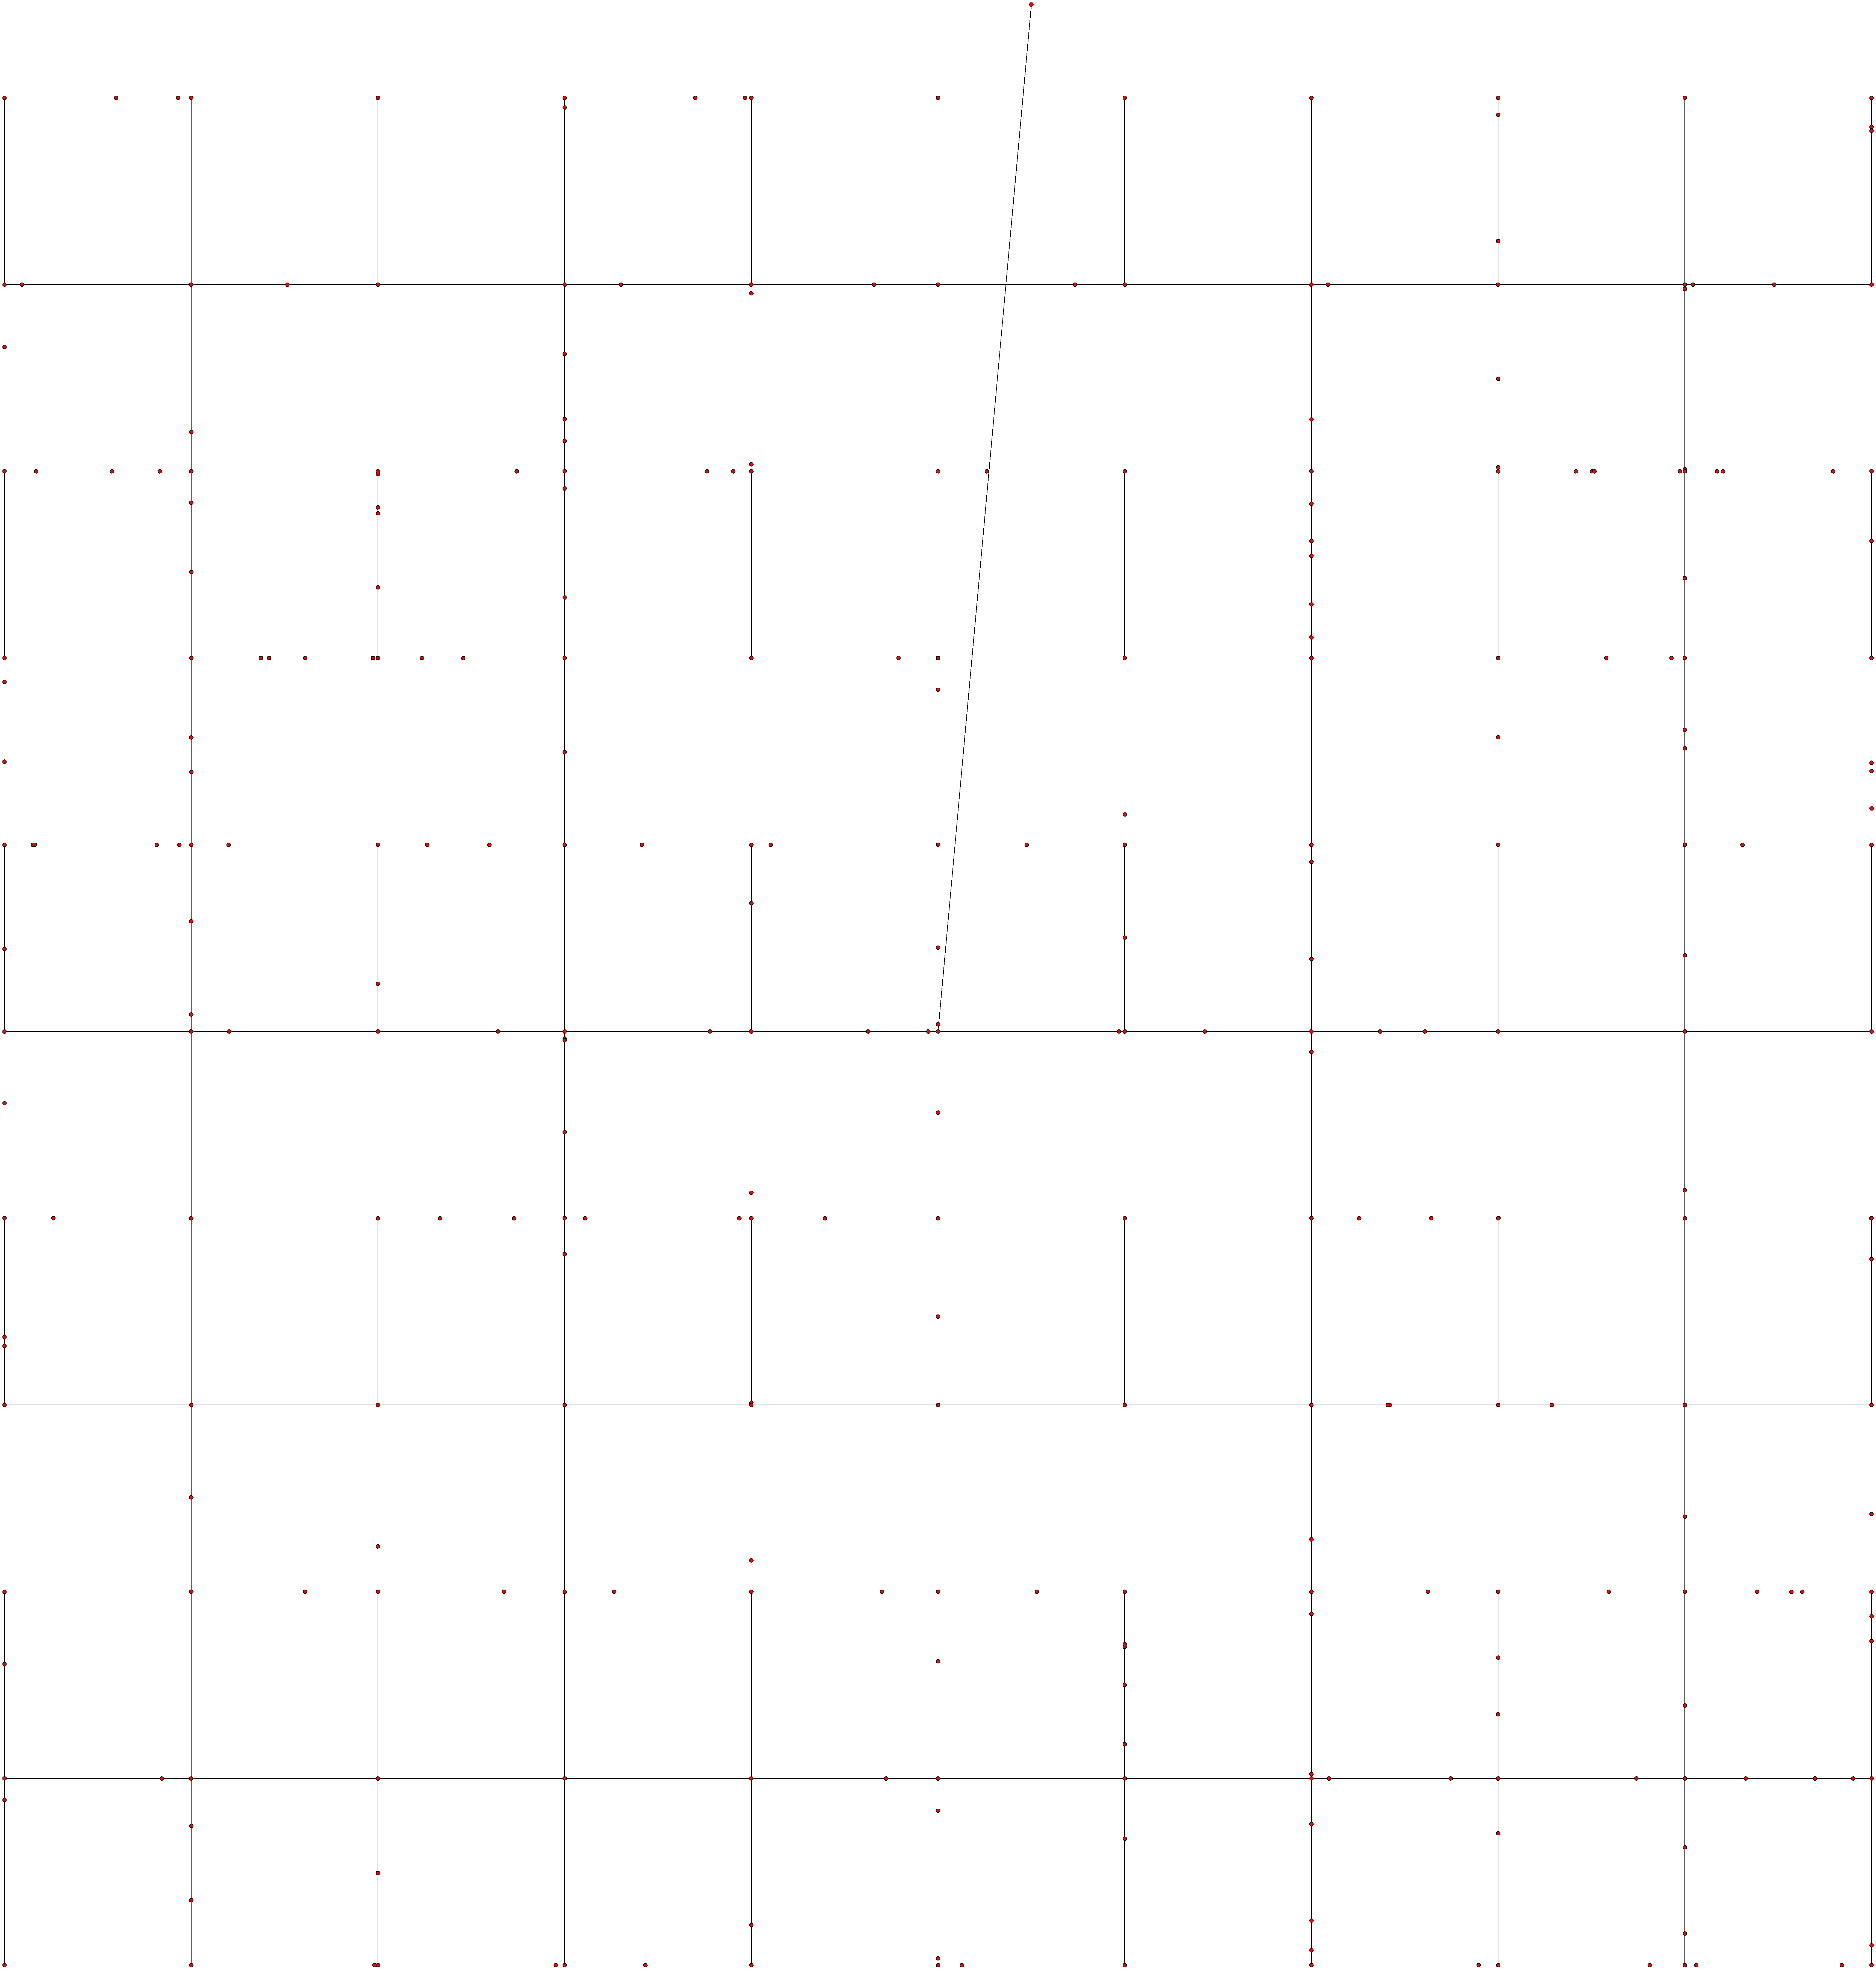
\includegraphics[width=3in]{manh2}
\caption{Access point position and connections on the Manhattan mobility
model.}\label{fig:manh}
\end{figure}

For this model 200 vehicles were used, configured to travel with a speed with
mean of 10 meters per second and standard deviation 0.2. Vehicles request
content with a frequency of 10 contents per second during the entire simulation,
each content has a name {\tt /prefix/k} where {\tt k} is a sequential index.
Each content is provided with a content size of 1024 bytes.

\section{Simulation Tools}\label{sec:simu}

The environment described in Section~\ref{sec:commmodel} was simulated with the
discrete event network simulator Netowrk Simulator 3 (ns-3)~\cite{ns3web}. More
specifically the nsnSIM module~\cite{mastorakis2015ndnsim} was used to emulate
the NDN network. Both ns-3 and ndnSIM are written in C++ and open source
distributed. The ndnSIM is a realistic and useful module because it uses the
NDN~\cite{zhang2010named} platform, i.e., ndn-cxx library (NDN C++ library with
eXperimental eXtensions)~\cite{ndnp} and then NDN Forward Daemon
(NFD)~\cite{afanasyev2014nfd}. Those modules are used in real systems,
communication with the Linux network stack and implementing a real NDN network.
So code produced by simulation can be used in real systems with no need to
rewrite.

For the generation of vehicles movements pattern the
BonnMotion~\cite{aschenbruck2010bonnmotion} tool was used. As stated in
Section~\ref{sec:commmodel} the tool was configured to generate movement
patterns according to the Manhattan mobility model. BonnMotion is written in
Java and distributed as a open source software, it can generate and analyse
mobility scenarios, and export them to network simulators like ns-2,
GloMonSim/QualNet, COOJA, and MiXiM. This work used ns-3, ns-3 is able to use
ns-2 scenarios which were exported by BonnMotion.

\section{Results}\label{sec:result}

The results were obtained from a simulation of 180 seconds, in which the
statistics for content retrieval consider the first 500 content obtained on
each node, which can for example represent a video streaming application. To
analyse different scenarios four cache configurations were used.  The first
assumes no cache on any of the nodes and is used as reference. The others
configuration used a 10, 100 and 1000 content store on each access point node.

Figure~\ref{fig:hop} shows the average hop count that each content used to be
retrieved in each of the cache configuration.
As expected the average hop count decreases with a
larger cache. And no big gains are obtained after the cache size is 100.
Figure~\ref{fig:hop} also shows that for the first count the hop count is
larger than the mean, this is expected since no cache is available when the
system starts. Another observation that can be made is that the standard
deviation of the hop count in the lower cache is bigger, this can be explained
by a changing cache content on the lower cache configuration, and of course for
a bigger cache the cache content is more stable.

\begin{figure}
\centering
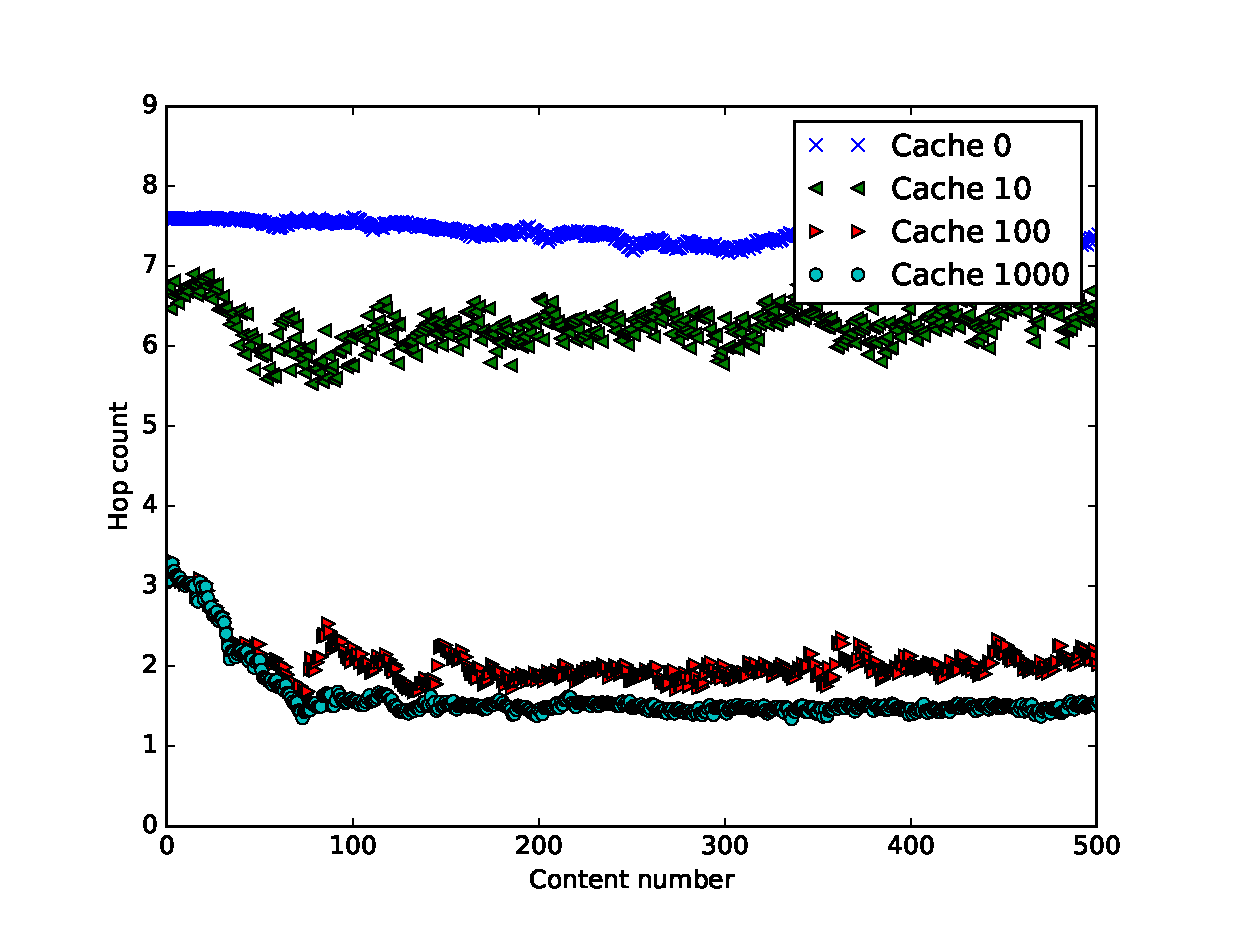
\includegraphics[height=2.6in]{hop}
\caption{Mean of hop count needed by each content with four cache
configurations.}\label{fig:hop}
\end{figure}

Table~\ref{tab:timediff} shows the mean of the difference between time in which
each content was retrieved in each node. It is shown that the higher the cache
the faster the content is retrieved, for example in average a content cache of
100 retrieve the content 4.6 faster than the environment with no cache.

\begin{table}[!t]
    \caption{Mean of the difference between time in which each content was
    retrieved in each node.}\label{tab:timediff}
    \centering
    \begin{tabular}{rcccc}
        \toprule
        & \bfseries Cache 0 & \bfseries Cache 10 & \bfseries Cache 100 &
            \bfseries Cache 1000 \\
        \midrule
        \bfseries Cache 0 & 0 & 0.6613 & 3.0542 & 3.8056 \\
        \bfseries Cache 10 & -0.6613 & 0 & 2.2930 & 3.1453 \\
        \bfseries Cache 100 & -3.0542 & -2.3930 & 0 & 0.7514 \\
        \bfseries Cache 1000 & -3.8056 & -3.1443 & -0.7514 & 0 \\
        \bottomrule
    \end{tabular}
\end{table}

In Figure~\ref{fig:last} the last delay per content in each cache configuration
is shown. The last delay is defined as the delay between the last request sent
and data packet received. Again the simulation show that with high cache a
small delay is obtained, and that there not much gain after 100 content cache.

\begin{figure}
\centering
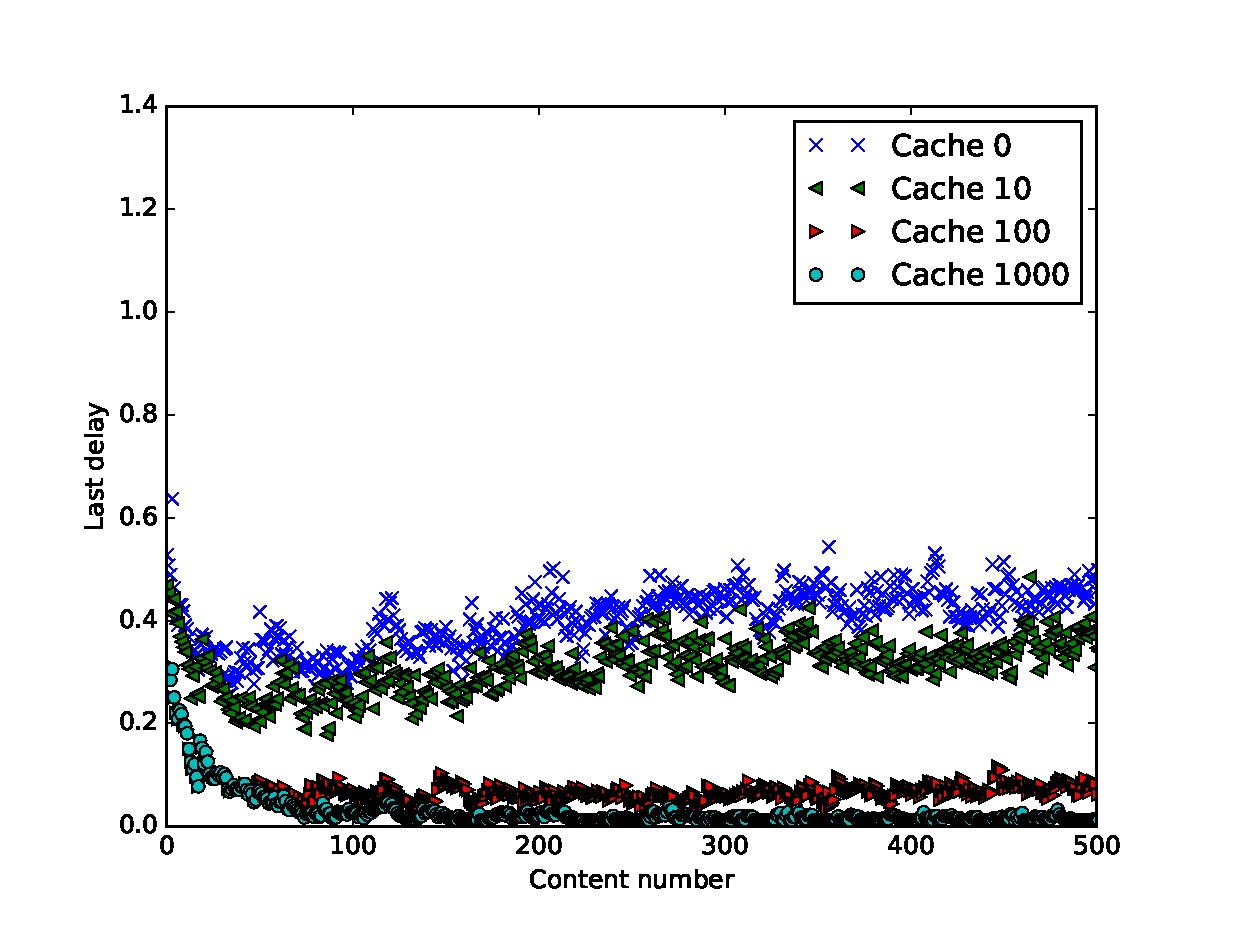
\includegraphics[height=2.6in]{last}
\caption{Last delay per content in each cache configuration.}\label{fig:last}
\end{figure}

To analyse the producer load Figure~\ref{fig:prodsatis} shows the satisfied
requests provided by the producer. It shows that with a higher cache its
content is less and less consulted, and there is still gain after the cache is
100 contents. This figure also infers that with a high cache the network
possess the content, and it can take care of deliver it to clients.

\begin{figure}
\centering
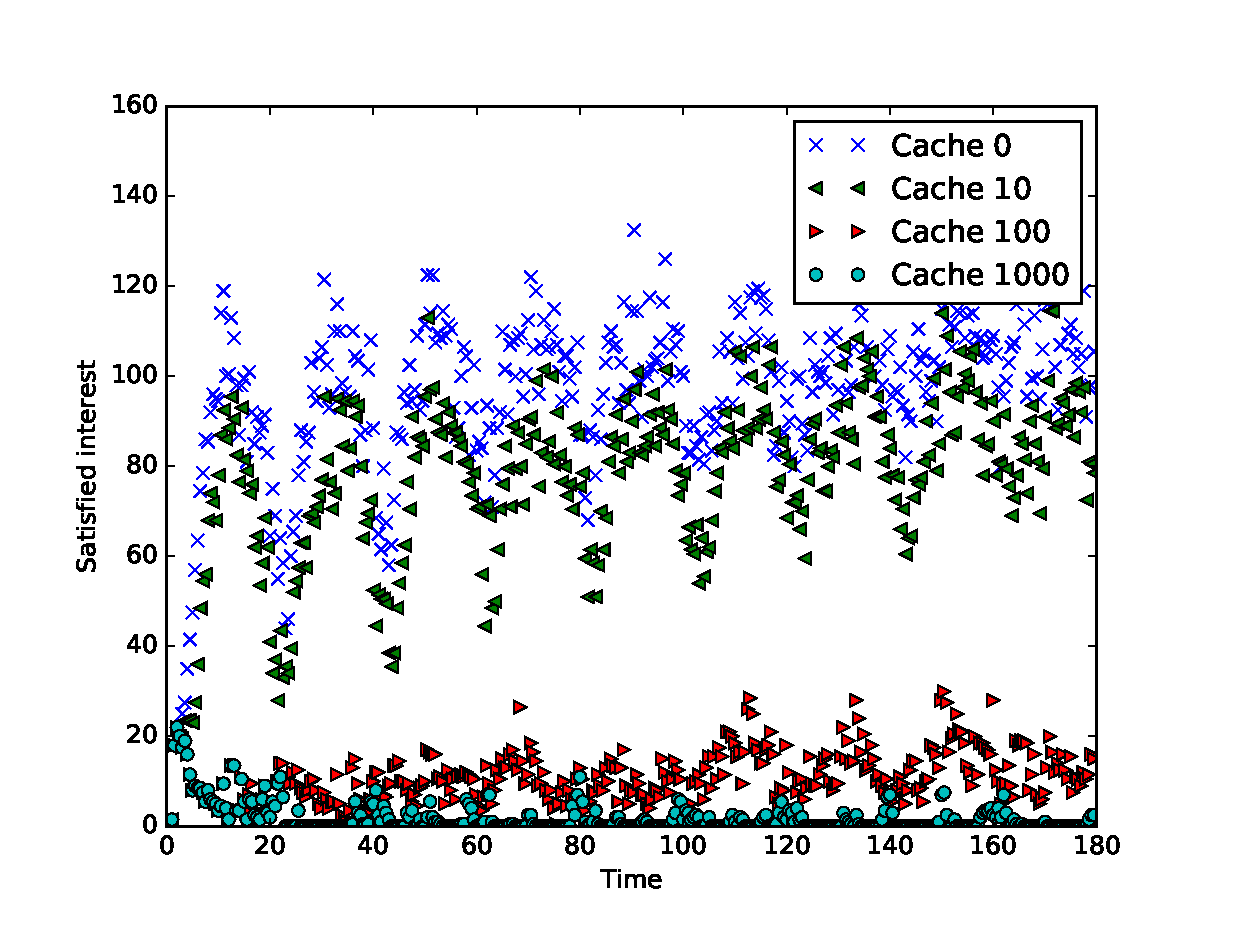
\includegraphics[height=2.6in]{prodsatis}
\caption{Satisfied request provided by the producer over
time.}\label{fig:prodsatis}
\end{figure}

Figure~\ref{fig:satisfied} validate the previous conclusions by showing that
with a larger cache more interests are satisfied per unit of type. This is, a
higher total throughput can be achievable.

\begin{figure}
\centering
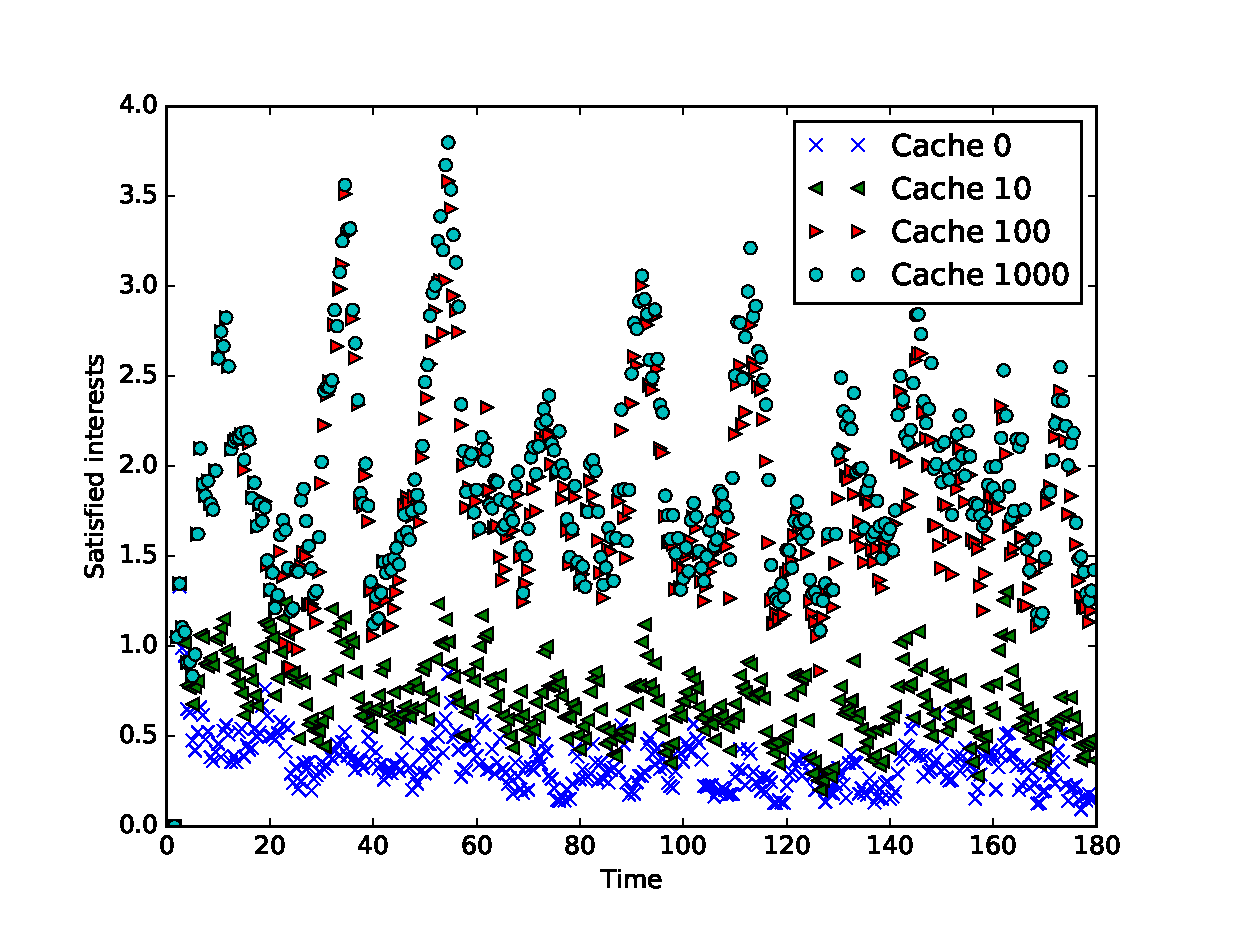
\includegraphics[height=2.6in]{satisfied}
\caption{Vehicles' satisfied interests average per time.}\label{fig:satisfied}
\end{figure}

\section{Conclusion and Future Works}\label{sec:conc}

It was shown that the cache is an important component of the NDN V2I network,
using cache it is possible not only to reduce network traffic, but also
increase server resources and provide a connection with a lower latency to the
user, so a more seamless experience is achievable.

It was a great challenge to use the ndnSIM, a lot of background on ns-3 is
assumed on its documentation, and some of them are not very great in detail.
The biggest difficulty was with the routing of the NDN network, it seems like
the default global routing algorithm of ndnSIM used to populate the FIB tables
are not working well for the proposed model. Further analyses is need to find
the problem, but for this work the FIB tables were manually populated.

As future work, the speed and number of vehicles should be further studied to
simulate an even more real system, mainly the standard deviation of the
vehicles speed. The proposed network topology is a tree, so the cache should
also be considered to be different on each layer of nodes (considering each
layer as the depth from the producer), perhaps using higher cache on lower
layers would produce similar results using less physical resources. Using the
proposed scenario is also possible to study the content retrieval of vehicles
producers, i.e., the case where producer and consumer are both vehicles.

\bibliographystyle{IEEEtran}
\bibliography{ref.bib}

\end{document}
